\begin{lemma}
Tangent to a circle : Consider a circle 
\begin{align}
    \vec{x}^\top\vec{x} + 2\vec{c}^\top\vec{x} + f = 0 
\end{align}
Given a point $\vec{q}$ on the circle, the tangent at that point is given as,
\begin{align}
    \brak{\vec{q}+\vec{c}}^\top\vec{x} + \vec{c}^\top\vec{q} + f = 0 
\end{align}
\end{lemma}
\begin{lemma}
Orthogonality of circles : Two circles are said to be orthogonal if  the tangents at their points of intersection are perpendicular to each other.\\ That implies, tangents to one circle at the points of contact are normals to the other circle. 
Given two circles,
\begin{align}
    \vec{x}^\top\vec{x} + 2\vec{c_1}^\top\vec{x} + f_1 = 0 \label{4/4/2/eq1}\\
    \vec{x}^\top\vec{x} + 2\vec{c_2}^\top\vec{x} + f_2 = 0 \label{4/4/2/eq2}
\end{align}
They are orthogonal if
\begin{align}
    2\vec{c_1}^\top\vec{c_2} = f_1 + f_2 \label{4/4/2/condition}
\end{align}
\end{lemma}
\begin{proof}
Let the two circles \eqref{4/4/2/eq1} and \eqref{4/4/2/eq2} meet at a point $\vec{q}$ i.e $\vec{q}$ satisfies the equation of the circles
\begin{align}
    \vec{q}^\top\vec{q} + 2\vec{c_1}^\top\vec{q} + f_1 = 0 \label{4/4/2/2.0.4}\\
    \vec{q}^\top\vec{q} + 2\vec{c_2}^\top\vec{q} + f_2 = 0 \label{4/4/2/2.0.5}
\end{align}
Eliminating quadratic term,
\begin{align}
    2\brak{\vec{c_1}^T - \vec{c_2}^T}\vec{q} + f_1 - f_2 = 0 \label{4/4/2/2.0.6}
\end{align}
Given the point of contact $\vec{q}$, the equation of tangent to circle \eqref{4/4/2/eq1} is
\begin{align}
    \brak{\vec{q}+\vec{c_1}}^\top\vec{x} + \vec{c_1}^\top\vec{q} + f_1 = 0 
\end{align}
As it is a normal to the second circle \eqref{4/4/2/eq2}, it passes through the center of it
\begin{align}
    \brak{\vec{q}+\vec{c_1}}^\top\brak{\vec{-c_2}} + \vec{c_1}^\top\vec{q} + f_1 = 0 \\
    \implies \brak{\vec{c_1}^T - \vec{c_2}^T}\vec{q} + f_1 - \vec{c_1}^T\vec{c_2} = 0 \\
    \implies \brak{\vec{c_1}^T - \vec{c_2}^T}\vec{q} = \vec{c_1}^T\vec{c_2} - f_1
    \label{4/4/2/2.0.10}
\end{align}
Substituting \eqref{4/4/2/2.0.10} in \eqref{4/4/2/2.0.6},
\begin{align}
    2\brak{\vec{c_1}^T\vec{c_2} - f_1}  + f_1 - f2 = 0 \\
    \implies 2\vec{c_1}^\top\vec{c_2} = f_1 + f_2 
\end{align}
\end{proof}
\begin{lemma}
For given three circles,
\begin{align}
    \vec{x}^\top\vec{x} + 2\vec{c_1}^\top\vec{x} + f_1 = 0 \label{4/4/2/S1=0}\\
    \vec{x}^\top\vec{x} + 2\vec{c_2}^\top\vec{x} + f_2 = 0 \label{4/4/2/S2=0}\\
    \vec{x}^\top\vec{x} + 2\vec{c_3}^\top\vec{x} + f_3 = 0 \label{4/4/2/S3=0}
\end{align}
The equation of a circle $S$ which cuts these circles orthogonally is given by,
\begin{align}
    \vec{x}^\top\vec{x} + 2\vec{c}^\top\vec{x} + f = 0 \label{4/4/2/S=0}
\end{align}
Where 
\begin{align}
    \myvec{\vec{c}\\f} = \myvec{2\vec{c_1}^\top&-1\\2\vec{c_2}^\top&-1\\2\vec{c_3}^\top&-1}^{-1}\myvec{f_1\\f_2\\f_3}
\end{align}
\end{lemma}\label{4/4/2/lemma2}
\begin{proof}
Since $S$ is orthogonal to \eqref{4/4/2/S1=0}, \eqref{4/4/2/S2=0} and \eqref{4/4/2/S3=0} we have,
\begin{align}
    2\vec{c_1}^\top\vec{c} - f &= f_1\\
    2\vec{c_2}^\top\vec{c} - f &=  f_2\\
    2\vec{c_3}^\top\vec{c} - f &= f_3\\
    \implies \myvec{2\vec{c_1}^\top&-1\\2\vec{c_2}^\top&-1\\2\vec{c_3}^\top&-1}\myvec{\vec{c}\\f} &= \myvec{f_1\\f_2\\f_3}\\
\end{align}
\end{proof}
Let the required equation of the circle be
\begin{align}
    \vec{x}^\top\vec{x} + 2\vec{c}^\top\vec{x} + f = 0
\end{align}
It is orthogonal to the circles \eqref{4/4/2/circle1}, \eqref{4/4/2/circle2} and \eqref{4/4/2/circle3}
\begin{align}
    \implies \myvec{4&-5&-1\\5&-6&-1\\-1&-1&-1}\myvec{\vec{c}\\f} = \myvec{6\\7\\-1}
\end{align}
Therefore the augmented matrix can be transformed as,
 \begin{align}
		\myvec{4 & -5 & -1 & 6\\
		       5 & -6 & -1 & 7\\
		       -1 & -1 & -1 &-1}\\
		\xleftrightarrow[]{R_1\leftrightarrow-R_3 }
		\myvec{1 & 1 & 1 & 1\\
		       5 & -6 & -1 & 7\\
		       4 & -5 & -1 & 6}\\
		\xleftrightarrow[R_2 \leftarrow R_2-5R_1, R_2 \leftarrow -\frac{R_2}{11}]{R_3 \leftarrow R_3-4R_1}
		\myvec{1 & 1 & 1 & 1\\
		       0 & 1 & \frac{6}{11} & \frac{-2}{11}\\
		       0 & -9 & -5 &2}\\
		\xleftrightarrow[R_1 \leftarrow R_1-R_2]{R_3 \leftarrow R_3+9R_2}
		\myvec{1 & 0 & \frac{5}{11} & \frac{13}{11}\\[0.2cm]
		       0 & 1 & \frac{6}{11} & \frac{-2}{11}\\[0.2cm]
		       0 & 0 & \frac{-1}{11} & \frac{4}{11}}\\
		\xleftrightarrow[R_1 \leftarrow R_1+5R_3, R_3 \leftarrow -11R_3]{R_2 \leftarrow R_2+6R_3}
		\myvec{1 & 0 & 0 & 3\\ 
		       0 & 1 & 0 & 2\\
		       0 & 0 & 1 &-4}\\
    \implies \vec{c} = \myvec{3\\2}, f = -4 		       
\end{align}

The required equation of circle,
\begin{align}
    S = \vec{x}^\top\vec{x} + \myvec{6&4}\vec{x} - 4 = 0
\end{align}
\begin{figure}[h!]
\centering
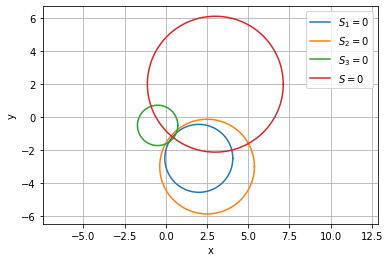
\includegraphics[width=\columnwidth]{solutions/4/4/2/figures/CirclesPlot.png}
\caption{Plot of circles}
\label{4/4/2/fig:circles plot}
\end{figure}

